\documentclass{article}
\usepackage[utf8]{inputenc}
\usepackage{graphicx}
\usepackage{caption}
\usepackage{float}

\title{Differential Compliance with Lockdown Policies: The Case of Netherlands}
\author{Yuxin Wang}
\date{March 2021}

\begin{document}

\maketitle

\section{Background}
The first positive COVID-19 case in the Netherlands was reported on February 27, 2020. In March 2020, the COVID-19 pandemic hit the Netherlands to its full extent. On March 12, after a sustained increase in the number of positive cases, and despite repeated calls for adherence to general hygiene measures like frequent hand-washing and not shaking hands, the government decided national lockdown restrictions were required to prevent further transmission of the virus. The prime minister, the head of the outbreak-management team (i.e., the scientific advisory board for COVID-19 prevention), and the minister for healthcare held a joint press conference and announced: (1) the prohibition of public and private events (100 attendees or more); (2) a request for everyone to work from home wherever possible; (3) limitations on visits to the elderly or those with medical conditions; and (4) a stay-at-home order in the event of respiratory problems or a fever. There was a further press conference on March 15, when it was announced that these measures would be complemented with an urgent request for social distancing of at least 1.5 m and the closure of schools, restaurants, gyms, and other related businesses. Restrictions on entering the country were also imposed on people from outside the EU undertaking non-essential travel. This marked the start of the lockdown in the Netherlands, which was to initially remain in place until April 6, 2020.


\section{Data}

The dataset used in this research is a survey from the Longitudinal Internet Studies for the Social Sciences (LISS) panel. The LISS panel is a Dutch survey of households that have been interviewed repeatedly for more than ten years on a broad variety of topics. The panel is based on a true probability sample of households drawn from the population register by Statistics Netherlands and consists of roughly 5,000 households, comprising about 7,000 individuals. Surveys are administered by CentERdata, a research institute affiliated with Tilburg University which is specialized in collecting, analyzing and disseminating data. 
A special CoViD-19 survey about behaviors, beliefs and expectations during the ongoing pandemic has been administered monthly to the members of the LISS panel. The first wave was fielded at the beginning of the lockdown in the Netherlands, between March 20th and 31st 2020. During the first month of the questionnaire, several questions were asked about various social distancing policies and the assessments of its effectiveness, support for and compliance with these policies. Therefore, we use the data from the first wave to see how compliance with policies differs according to sociodemographic variables. All questions from the surveys are documented at the CoViD-19 Impact lab (2020).

Given the restriction the total number of households in the selected sample is 971, which consist of 1094 observations in the first wave.
Selections on question 3 (Social Distancing) and question 10 (Compliance with Curfew) are aimed to generate compliance index for each individual. For people who don’t stay at home in question 10 and don’t follow any recommendations in question 3, we directly set their compliance index to zero. Given 6 recommendations on social distancing in question 3, one way to measure the level of compliance is by summing up the number of recommendations each individual followed.
Background variables are presented in Table 1.

\section{Result}


By merging the dataset in the first wave survey and background data together, it’s possible to first look at the correlations between compliance with policies and different sociodemographic variables, as shown in Table 2. Education level is positively correlated with compliance index, meaning that the higher educated group tends to obey the rules in a greater extent. Number of household members, number of living-at-home children in the household and domestic situation are all positively correlated with compliance index as well, which shows that people with more members living together will be more compliant and avoid getting infected than the single ones. Urban character of place of residence is also depicted in Table 2, it measures the surrounding address density per km2 and is also positively correlated with compliance index. People living in a higher address density are more likely to disobey the lockdown policies than those live in outskirts.


A simple OLS regression is used in Table 3.
The regression function is:
$$
y_i = x_i \beta_1 + \beta_2*gender + \beta_3 *dom\_situation + \beta_4*hh\_members + \epsilon_i
$$
,where $y_i$ is the compliance index we generate from the first wave survey, $x_i$ are variables depicting age and education level. Gender is a dummy which equals to 1 when the individual is female and 0 for male. $dom_situation$ is a dummy equaling 0 when the domestic situation of an individual is single and 1 otherwise. $hh_members$ is a dummy which equals to 0 if the person don't have any family members and 1 otherwise. Each observation is subscripted for the individual $i$.

Noticing that the coefficient of age is negative, which seems to be opposite to our expectation, we visualize the relationship between age and compliance index in Figure 1. The result in Figure 2 is the same by dividing age group into three categories (\textless{40}, 40 to 65, \textgreater{65}). To have more fine-grained age groups, we divide age into 10 categories and visualize the result in Figure 3. We find that people who are below 20 years old and between 70 to 89 years old are less compliance with the lockdown policies. The regression results are shown in Table 4.


Moreover, both male and female are compliant with the lockdown policy, but female show a higher level of compliance than male, with their coefficients of 0.647 and 0.443 respectively.
The education level is divided into five categories, however, all observations have primary school level or university degree. As shown in Table 4, education level is positively correlated with policy compliance. As education level increases from primary school to university degree, compliance index goes up 0.09 unit. The result can be also explained because primary school students are below 20 years old and it is the same result as we can see from age group division.
Number of household members and domestic situation are also included in Table 4. It shows that the more members are in one household, the higher level of compliance with policies individual will have than the single ones.



\begin{table}[h]
\centering
\caption{Background Variables}
\label{table:value_counts}
\begin{tabular}{ll}
\hline
variable                                                                           & counts \\ \hline
Gender                                                                      &        \\
male                                                                             & 542    \\
female                                                                             & 536    \\ \hline
age\_group\_by10                                                                &        \\
0 - 9                                                                           & 0      \\ 
10 - 19                                                                         & 111    \\
20 - 29                                                                         & 173    \\
30 - 39                                                                         & 168    \\
40 - 49                                                                         & 132    \\
50 - 59                                                                         & 123    \\
60 - 69                                                                         & 170    \\
70 - 79                                                                         & 156    \\
80 - 89                                                                         & 38     \\
90 - 99                                                                         & 7      \\ \hline
Education Level                                                                  &        \\
university                                                                      & 696    \\
primary school                                                                  & 382    \\
other                                                                           & 0      \\\hline
Domestic Situation                                                                  &        \\
(un)married co-habitation, without child(ren)                                   & 349    \\
(un)married co-habitation, with child(ren)                                      & 341    \\
single                                                                          & 294    \\
single, with child(ren)                                                         & 55     \\
other                                                                           & 39     \\ \hline
Number of Household Members                                                                     &        \\

1.0                                                                             & 294    \\
2.0                                                                             & 392    \\
3.0                                                                             & 106    \\
4.0                                                                             & 162    \\
5.0                                                                             & 89     \\
6.0                                                                             & 23     \\
7.0                                                                             & 11     \\
9.0                                                                             & 1      \\ \hline
Number of Household Children                                                    &        \\
0.0                                                                             & 682    \\
1.0                                                                             & 113    \\
2.0                                                                             & 168    \\
3.0                                                                             & 85     \\
4.0                                                                             & 19     \\
5.0                                                                             & 11     \\ \hline
Location Urban                                                                  &        \\
extremely urban                                                                 & 281    \\
very urban                                                                      & 240    \\
moderately urban                                                                & 176    \\
slightly urban                                                                  & 187    \\
not urban                                                                       & 194    \\ \hline
\end{tabular}
\end{table}


\begin{table}[h]
\centering
\caption{Correlations}
\label{table:correlations}
\begin{tabular}{lllllllll}
\hline
                       & ci    & age    & gender & hh\_member & hh\_children & urban & dom\_situation & edu \\ \hline
comliance index                    & 1.0    & -0.164 & 0.081  & 0.043       & 0.042               & 0.039                  & 0.04                  & 0.198      \\
age                    & -0.164 & 1.0    & -0.129 & -0.385      & -0.424              & -0.087                 & -0.129                & -0.04      \\
gender                 & 0.081  & -0.129 & 1.0    & 0.006       & 0.027               & 0.04                   & -0.016                & -0.082     \\
hh\_members            & 0.043  & -0.385 & 0.006  & 1.0         & 0.78                & -0.188                 & 0.642                 & -0.116     \\
hh\_children    & 0.042  & -0.424 & 0.027  & 0.78        & 1.0                 & -0.159                 & 0.467                 & -0.107     \\
location\_urban & 0.039  & -0.087 & 0.04   & -0.188      & -0.159              & 1.0                    & -0.191                & 0.153      \\
dom\_situation  & 0.04   & -0.129 & -0.016 & 0.642       & 0.467               & -0.191                 & 1.0                   & -0.04      \\
education             & 0.198  & -0.04  & -0.082 & -0.116      & -0.107              & 0.153                  & -0.04                 & 1.0        \\ \hline
\end{tabular}
\end{table}

\begin{table}[h]
\centering
\caption{Regression 1}
\label{table:age_square}
\begin{tabular}{lllllll}
\hline
                       & coef    & std err & t      & P\textgreater{}\|t\| & {[}0.025 & 0.975{]} \\ \hline
const                  & 2.7160  & 0.277   & 9.821  & 0.000              & 2.173    & 3.259    \\
age                    & 0.0100  & 0.012   & 0.843  & 0.399              & -0.013   & 0.033    \\
age\_square            & -0.0002 & 0.000   & -1.723 & 0.085              & -0.000   & 2.93e-05 \\
edu\_index             & 0.1003  & 0.019   & 5.232  & 0.000              & 0.063    & 0.138    \\
female                 & 0.2177  & 0.082   & 2.647  & 0.008              & 0.056    & 0.379    \\
dom\_situation\_index  & 0.0613  & 0.052   & 1.177  & 0.239              & -0.041   & 0.164    \\
hh\_members\_dummy     & 0.0613  & 0.052   & 1.177  & 0.239              & -0.041   & 0.164    \\
hh\_children\_dummy    & -0.0803 & 0.107   & -0.751 & 0.453              & -0.290   & 0.129    \\
location\_urban\_index & -0.0062 & 0.029   & -0.212 & 0.832              & -0.064   & 0.051    \\ \hline
\end{tabular}
\end{table}




\begin{table}[h]
\centering
\caption{Regression 2}
\label{table:age_by10_index_cube}
\begin{tabular}{lllllll}
\hline
                         & coef    & std err & t      & P\textgreater{}\|t\| & {[}0.025 & 0.975{]} \\ \hline
const                    & 1.0896  & 0.432   & 2.520  & 0.012              & 0.241    & 1.938    \\

male                     & 0.4427  & 0.217   & 2.037  & 0.042              & 0.016    & 0.869    \\
female                   & 0.6469  & 0.223   & 2.904  & 0.004              & 0.210    & 1.084    \\

age\_by10\_index         & 0.9222  & 0.425   & 2.171  & 0.030              & 0.089    & 1.756    \\
age\_by10\_index\_square & -0.1815 & 0.081   & -2.244 & 0.025              & -0.340   & -0.023   \\
age\_by10\_index\_cube   & 0.0098  & 0.005   & 2.051  & 0.041              & 0.000    & 0.019    \\
edu\_index               & 0.0899  & 0.020   & 4.443  & 0.000              & 0.050    & 0.130    \\
dom\_situation\_index    & 0.0672  & 0.052   & 1.287  & 0.198              & -0.035   & 0.170    \\
hh\_members\_dummy       & 0.0672  & 0.052   & 1.287  & 0.198              & -0.035   & 0.170    \\
\hline
\end{tabular}
\end{table}




\clearpage

\begin{figure}[h]
\centering
\caption{Age}
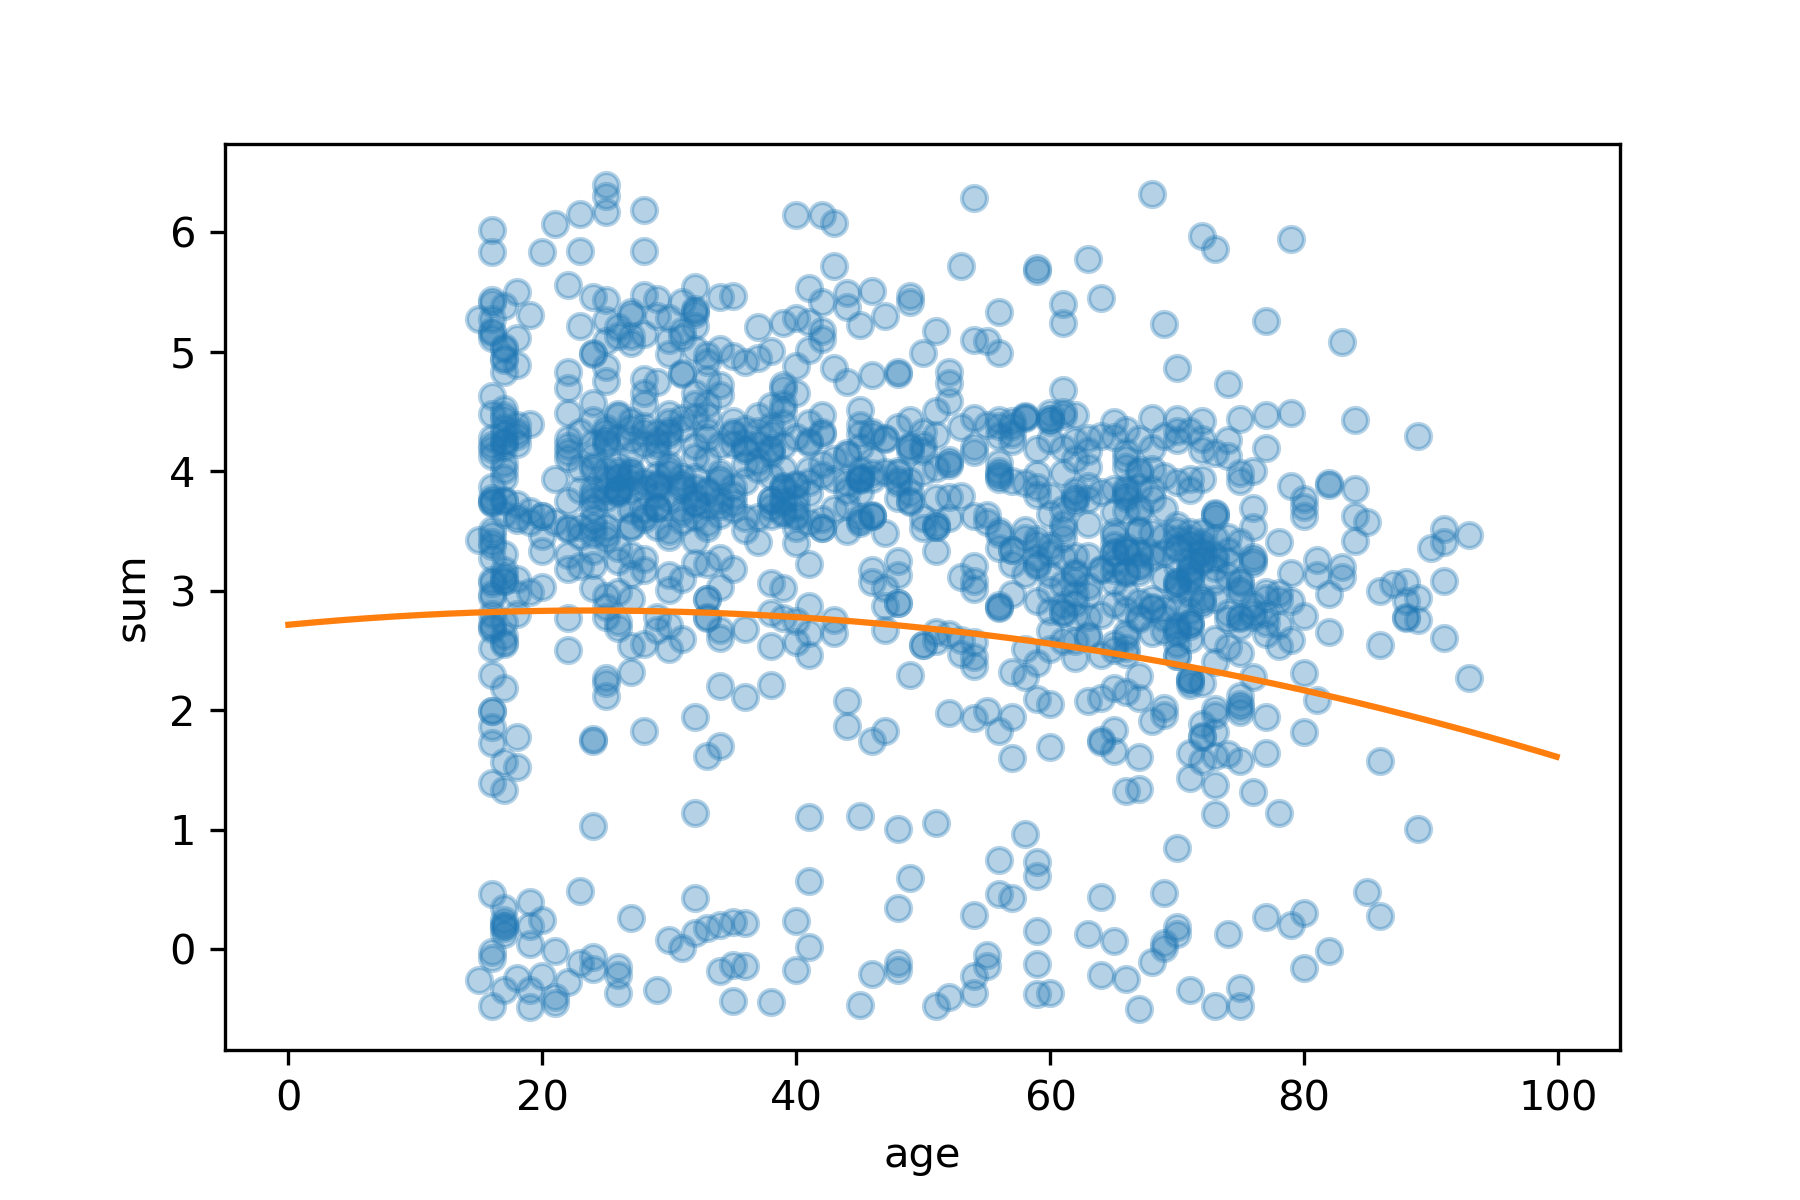
\includegraphics[width=1\textwidth]{figures/age_square.png}
\label{figure:age_square}
\end{figure}

\begin{figure}[h]
\centering
\caption{Age\_three groups}
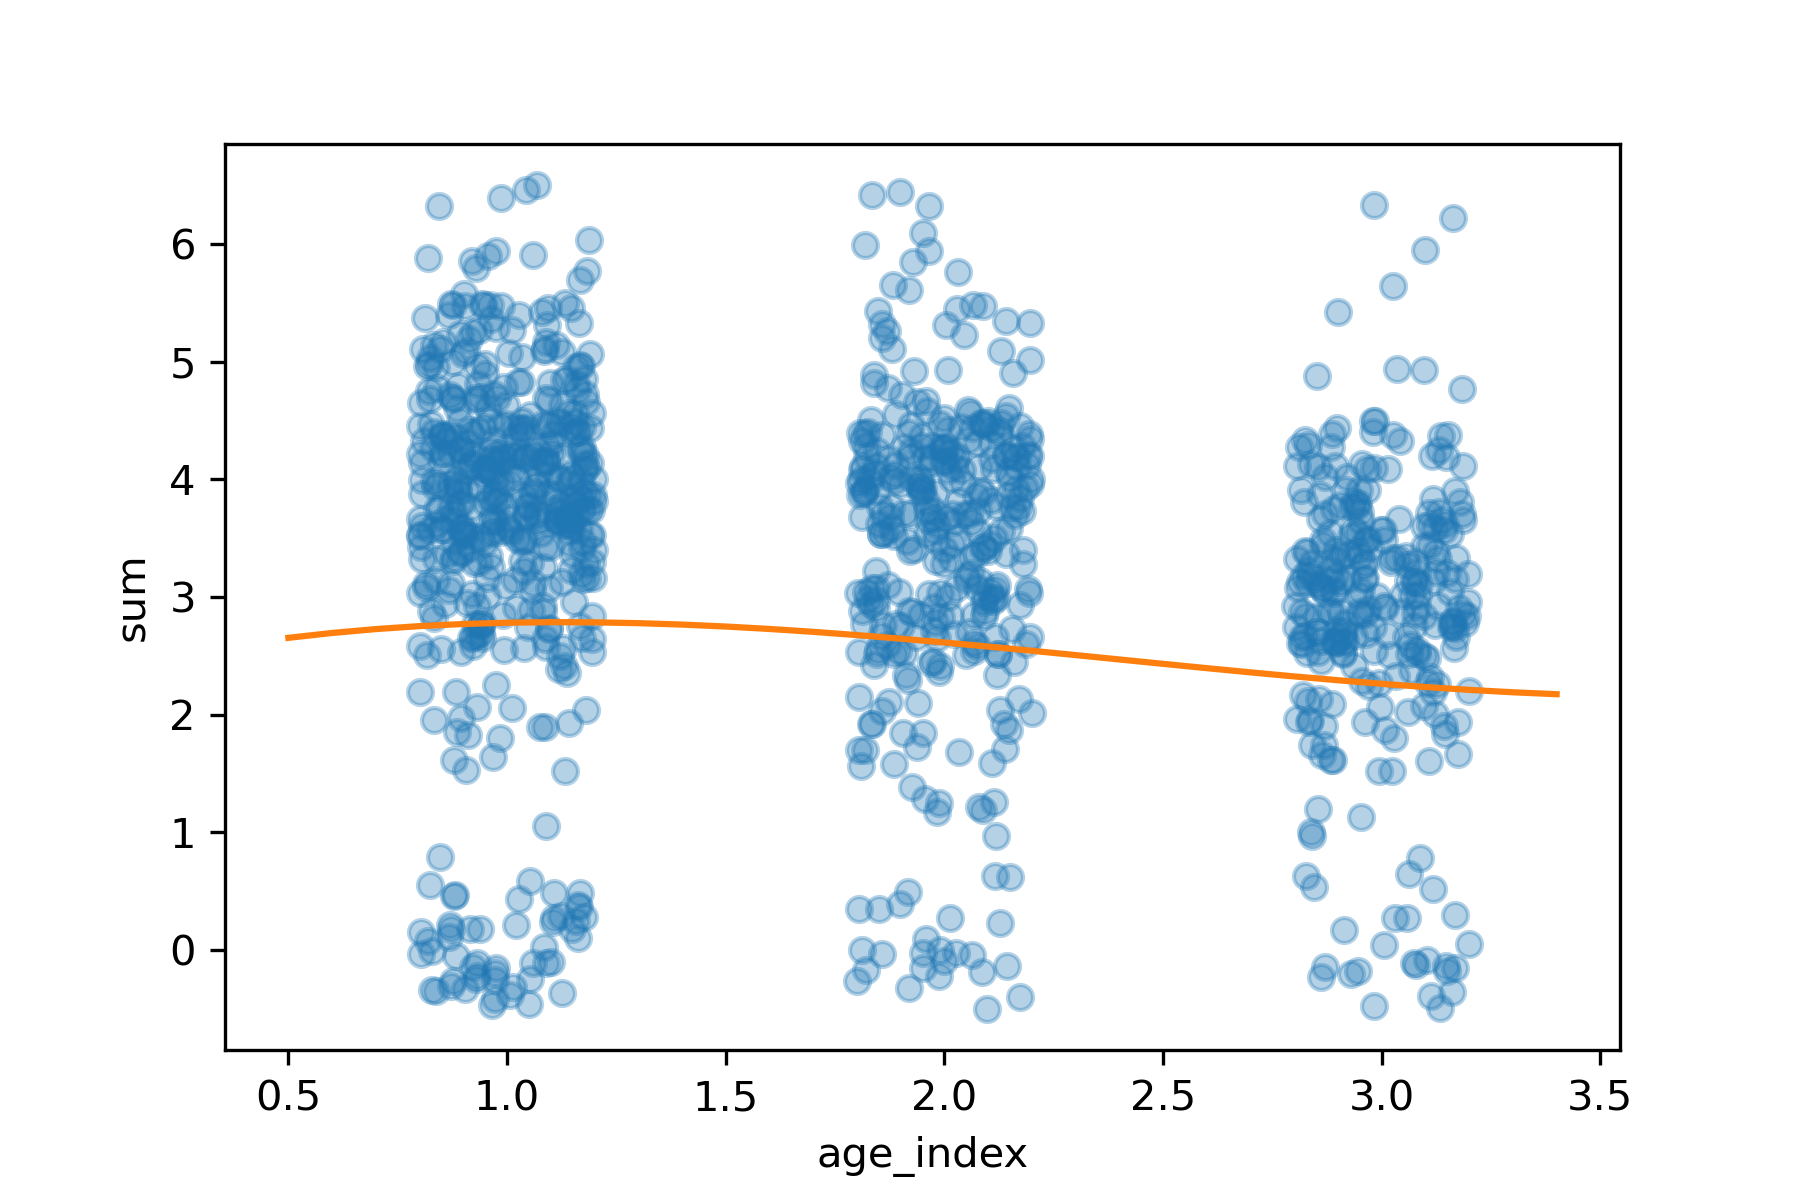
\includegraphics[width=1\textwidth]{figures/age_index_cube.png}
\label{figure:age_index_cube}
\end{figure}

\begin{figure}[h]
\centering
\caption{Age\_ten groups}
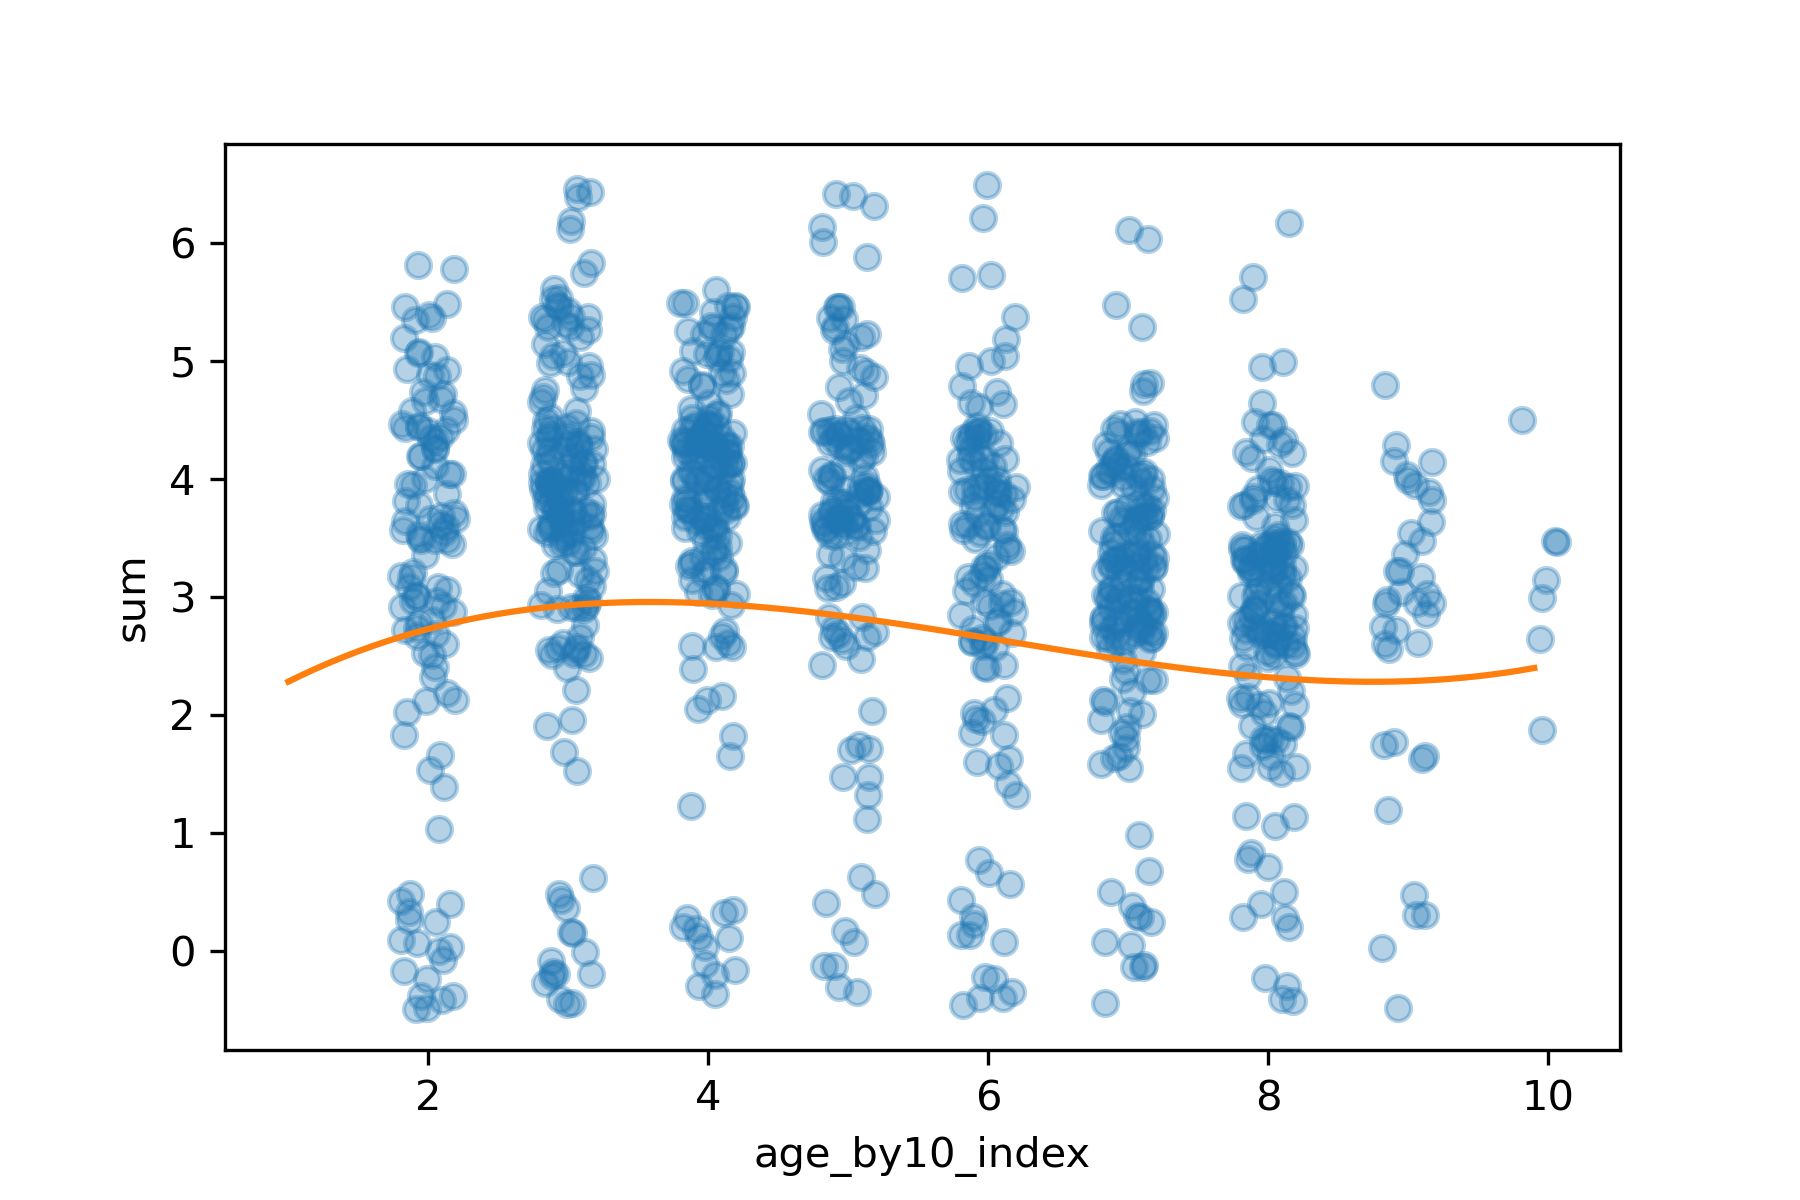
\includegraphics[width=1\textwidth]{figures/age_by10_index_cube.png}
\label{figure:age_by10_index_cube}
\end{figure}

\end{document}
